\documentclass[utf8, xcolor=dvipsnames]{beamer}

%\usepackage{default}
%\usepackage{beamerthemesplit}
%\usepackage{beamerthemeAnnArbor}
% \usepackage{beamerthemeAntibes}
% \usepackage{beamerthemeBergen}
% \usepackage{beamerthemeBerkeley}
% \usepackage{beamerthemeBerlin}
% \usepackage{beamerthemeBoadilla}
% \usepackage{beamerthemeboxes}
% \usepackage{beamerthemeCambridgeUS}
% \usepackage{beamerthemeCopenhagen}
% \usepackage{beamerthemeDarmstadt}
% \usepackage{beamerthemedefault}
% \usepackage{beamerthemeDresden}
% \usepackage{beamerthemeFrankfurt}
% \usepackage{beamerthemeGoettingen}
% \usepackage{beamerthemeHannover}
% \usepackage{beamerthemeIlmenau}
% \usepackage{beamerthemeJuanLesPins}
% \usepackage{beamerthemeLuebeck}
% \usepackage{beamerthemeMadrid}
% \usepackage{beamerthemeMalmoe}
% \usepackage{beamerthemeMarburg}
% \usepackage{beamerthemeMontpellier}
% \usepackage{beamerthemePaloAlto}
% \usepackage{beamerthemePittsburgh}
% \usepackage{beamerthemeRochester}
% \usepackage{beamerthemeSingapore}
% \usepackage{beamerthemeSzeged}
% \usepackage{beamerthemeWarsaw}
\usepackage{beamerthemeFreiburg}

% Color scheme blau oder anders?
\usecolortheme[named=Blue]{structure}
% \usecolortheme{wolverine}
\setbeamercolor{block title}{fg=craneblue,bg=craneorange}

% Mit oder ohne Schatten?
\setbeamertemplate{blocks}[rounded][shadow=false]

%\usepackage{pstricks}
\usepackage{german}
\usepackage{ragged2e}

%% zum Drucken:
% \usepackage{pgfpages}
% \pgfpagesuselayout{resize to}[a4paper,border shrink=5mm,landscape]
% \pgfpagesuselayout{2 on 1}[a4paper,border shrink=5mm]
% \pgfpagesuselayout{4 on 1}[a4paper,border shrink=5mm,landscape]
% \pgfpagesuselayout{8 on 1}[a4paper,border shrink=5mm]
% \pgfpagesuselayout{16 on 1}[a4paper,border shrink=5mm,landscape]
\renewcommand{\t}[1]{\texttt{#1}}


\title[Ethersex]{Das Ethersex-Projekt}
\subtitle{Einführung}
\author[RayVey]{Stesie \and Stettberger\newline \texttt{ethersex-devel@list.zerties.org}}
\date[EaHegg 10]{Easterhegg 2010}

\titlegraphic{
\includegraphics[width=0.5cm]{gnu-fdl.png}}
%FIXME \logo{
\includegraphics[width=1.5cm]{./bunnies-bg.png}}

\begin{document}

\frame{
  \frametitle{Ethersex}
  \titlepage
}

\frame{
  \frametitle{Übersicht}
  \tableofcontents[pausesections]
}

\frame{
  \begin{block}<1->{Zitat}
    \begin{quote}
      \justifying{
	Der Urquell aller technischen Errungenschaften
	ist die göttliche Neugier und der Spieltrieb des bastelnden und grübelnden Forschers
	und nicht minder die konstruktive Fantasie des technischen Erfinders...\\
	(A. Einstein: Eröffnung IFA 1930)
      }
    \end{quote}
  \end{block}
  \begin{block}<2->{Zusatz}
    \begin{quote}
      \justifying{
	... und Softwareentwicklers.
      }
    \end{quote}
  \end{block}
}

% Vortrag in 3 Teilen: Über Ethersex, Ethersex benutzen, Für Ethersex entwickeln

% Historie, Überblick (Kenndaten, Was macht das Projekt besonders), Abstraktionen (IO, Metaschicht, Kommunikation[ECMD]), 
\section{Über Ethersex}

% Einle
\subsection{Überblick}
\frame{
  \frametitle{Überblick}
  \begin{itemize}
    \item Zielplattform: Atmel AVR 8-Bit Mikrocontroller\pause
    \item Quellcode in C, ergänzt durch Präprozessor m4 \pause
    \item Dateien: $>1000$ \footnote<3->{Ermittelt mit: find . -type f $\mid$ grep -v git $\mid$ wc -l}
    \item Lines of Code: $\sim73832$ \footnote<3->{Ermittelt mit: find . -name ``*.[hc]'' $\mid$ xargs cat $\mid$ wc -l} \pause
    \item Modularer Aufbau: 93 Module
  \end{itemize}
  \pause
  \begin{block}{Komfort}
    \begin{itemize}
      \item Menü gesteuerte Auswahl von Zielhardware und Modulen
    \end{itemize}
  \end{block}
  \pause
  \begin{block}{Schnell erweiterbar}
    \begin{itemize}
      \item Eigenes Modul ohne Kenntnis des gesamten Quellcodes
      \item Gut dokumentiert (fast 100 Seiten Doku, Beispiele) % Habe hier die Wiki Seiten mit ethersex Kategorie gezählt (waren 93)
    \end{itemize}
  \end{block}
}

\frame{
  \frametitle{-v Zielplatform}
  \begin{itemize}
    \item Programmspeicher (Flash): 8Kb - 64Kb\pause
    \item RAM: 1 Kb - 4 Kb \pause
    \item Kosten pro Chip: 1 EUR - 10 EUR\pause
    \item Auswahl der Hardware über Menuconfig \pause
    \item Fast alle Module auf allen Prozessoren verfügbar
  \end{itemize}
}

%TODO Hier noch Zeitleiste einfügen
\subsection{Historie}
\frame{
  \frametitle{Die Entstehungsgeschichte}
  \begin{block}{Die Anfänge}
    \begin{itemize}
      \item<1-> August 2006: fd0 startet Etherrape für u23
      \item<2-> August 2007: stesie implementiert IPv6, Ethersex wird geforked
      \item<3-> Oktober 07: IP über RFM12 wird implementiert, weitere Netzwerkinterfaces folgen
      \item<4-> November 07: OpenVPN mit symmetrischer Krypto
    \end{itemize}
  \end{block}
}

\subsection{Ethersex Core}
\frame{
  \frametitle{Kerntech\^WBUZZWORD}
  \begin{block}{Menuconfig}
    \begin{itemize}
      \item Konfiguration mit Modulabhänigkeiten
      \item Übernommen vom Linuxkernel
      \item ncurses Interface (DEMO!)
    \end{itemize}
  \end{block}
  \pause
  \begin{block}{Pinning Abstraktion}
    \begin{itemize}
      \item Ordnet Pins einen Namen zu und ermöglicht Zugriff\pause
      \item \t{PIN(RED\_BUTTON, PB1)} - Definition eines Pins
      \item \t{PIN\_SET(RED\_BUTTON)} - Pin auf 5V setzen\pause
      \item Einfaces Verlegen von Anschlüssen\pause
      \item M4 powered        
    \end{itemize}
  \end{block}
}


\frame{
  \frametitle{Arbeitserleichterungen}
  \begin{block}{Ethersex META}
    \begin{itemize}
      \item Einzelnes Modul (Ordner) beinhaltet alles Notwendige\pause
      \item Sektion in der .c - Datei\pause
      \item Bsp. \texttt{periodic(meine\_periodic\_func, 50)}
      \item Funktion \t{meine\_periodic\_func} wird jede Sekunde (50 * 20ms) \
        aufgerufen\pause
      \item sed ... $\mid$ m4 ... $>$ meta.c
    \end{itemize}
  \end{block}
  \pause
  \begin{block}{Weiteres Basiszeugs}
    \begin{itemize}
      \item USART Abstraktion für die Auswahl Serieller Schnittstellen
      \item EEPROM Abstraktion für persistente Informationen
      \item Virtuelles Filesystem
    \end{itemize}
  \end{block}
}

%% \subsubsection*{IO Abstraktion}
%% \frame{
%%   \frametitle{IO Abstraktion}
%%   TODO Hier Quellcode
%% }

%% \subsubsection*{Metaschicht}
%% \frame{
%%   \frametitle{Metaschicht}
%%   TODO Hier Quellcode
%% }

\subsubsection*{Virtual File System}
\frame{
  \frametitle{Virtual File System}
  \begin{itemize}
    \item Verschiedene Backends (SD Karte, Interner Flash, Externer Dataflash)
    \item *nix like interface\pause
    \item \t{vfs\_file\_handle\_t fd = vfs\_open(``log'');}\\
      \t{vfs\_fseek(fd, 23, SEEK\_CUR);}\\
      \t{vfs\_read(fd, buf, 42);}\\
      \t{vfs\_close(fd);}
  \end{itemize}
}

\subsection{Modularer Aufbau}
\frame{
  \frametitle{Die Module}
  \begin{block}{Klar gegliedert}
    \begin{itemize}
      \item Hardware Module
      \item Protokoll Module
      \item Service/Anwendungs Module
    \end{itemize}
  \end{block}

  \pause

  \begin{block}{Komfort}
    \begin{itemize}
      \item Menü gesteuerte Auswahl der Module \pause
      \begin{itemize}
	\item Kleiner, performanter Code für den $\mu$Prozessor
      \end{itemize}
    \end{itemize}
  \end{block}
}

\subsection{Kommunikation}
%TODO Hier muss noch ecmd erklärt werden
\frame{
  \frametitle{Steuerungsprotokoll ECMD}
  \begin{itemize}
  \item ECMD als zentrale Interaktionsschnittstelle\pause
  \item Einzeilige ASCII Kommandos, ähnlich Shell\pause
  \item Bsp.: \t{io get pin 0}
  \item Holt den Eingangsstatus für Port 0 \\
    (PORTA oder PORTB je nach Prozessor)
  \end{itemize}
}

\frame{
  \frametitle{Steuerungsprotokoll ECMD}
  Zugriff auf die ECMD Schnittstelle über: \pause
  \begin{itemize}
  \item Per Netzwerk \pause
	\begin{itemize}
	\item TCP (HTTP Protokoll)
	\item TCP
	\item UDP\pause
    \item Jabber
    \item IRC\pause
    \item HTTP ( + Javascript = Dynamische Webseiten)
    \end{itemize} \pause
  \item Per USB \pause
  \item Per I2C \pause
  \item Per RS232/RS485 \pause
  \item $\cdots$
  \end{itemize}
}

%TODO Hier noch Module rauspicken und erläutern
% Rayofhope/david: Ich würde hier Stella Softpwm und Cron/Dynamic Cron nehmen
\subsection{Modulübersicht}
% \subsubsection{Netzwerk-anbindung}
\frame{
\frametitle{Ethersex features}
\begin{block}{Netzwerkanbindung}
\begin{itemize}
  \item Ethernet (ENC28J60) inkl. IEEE 802.1q (VLANs)
  \item USB (Software USB, Userland TUN Treiber)
  \item RFM12 (Funkübertragung auf dem 433 MHz ISM-Band)
  \item ZBus - Eigenes Protokoll für serielle Schnittstelle
\end{itemize}
\end{block}
}

% \subsubsection{Interaktion mit dem Anwender}
%% \frame{
%% \frametitle{Ethersex features}
%% \begin{block}{Interaktion mit dem Anwender}
%% \begin{itemize}
%%   \item HTTP-Server (mit Zugriff auf Dateien und ECMD)
%%   \item text-basiert (Telnet-ähnlich, TCP/IP oder UDP/IP)
%%   \item über serielle Schnittstelle
%%   \item über I2C
%%   \item via Jabber/XMPP
%%   \item via IRC
%% \end{itemize}
%% \end{block}
%% }

% \subsubsection{Netzwerkprotokolle}
\frame{
\frametitle{Ethersex features}
\begin{block}{Netzwerkprotokolle}
\begin{itemize}
  \item TCP/IP, UDP/IP und ICMP
  \item BOOTP (einfacherer, besser geeigneterer, Vorgänger von DHCP, der jedoch von allen gängigen DHCP-Servern unterstützt wird)
  \item TFTP (Upload von Firmwaredateien bzw. in den Data Flash Baustein)
  \item SYSLOG
  \item SNMP
  \item SMTP (E-Mail-Versand)
  \item NTP (Client und Server)
  \item DNS
\end{itemize}
\end{block}
}
\frame{
\frametitle{Ethersex features}
\begin{block}{Netzwerkprotokolle}
\begin{itemize}
  \item mDNS (Avahi)
  \item DynDNS
  \item MySQL (Client)
  \item IRC (Client)
  \item MPD (Music Player Daemon; einfache Steuerungsaufgaben)
  \item SOAP/XMLRPC
  \item UPnP
\end{itemize}
\end{block}
}

% \subsubsection{Kontakt zur Außenwelt}
% \frame[allowframebreaks]{
\frame{
\frametitle{Ethersex features}
\begin{block}{Kontakt zur Außenwelt}
\begin{itemize}
  \item RS232 und RS485
  \item Infrarotsender und -empfänger (RC5 Fernbedienungen!)
  \item I2C (Master und Slave)
  \item Steuerung von FS20-Modulen (Funkmodule von ELV bzw. Conrad, u.a. Steckdosen, Dimmer und Temperatursensoren)
  \item Modbus
  \item YPort (Serial over LAN (SOL) auch als XPort bekannt)
  \item Blinkenlights MCUF
  \item Porterweiterungen durch HC595 und HC165 möglich
\end{itemize}
\end{block}
}
\frame{
\frametitle{Ethersex features}
\begin{block}{Kontakt zur Außenwelt}
\begin{itemize}
  \item Dateneingabe mittels PS/2 Tastatur
  \item Dallas 1-wire Bus
  \item LCD (HD44780 und Kompatible)
  \item Philips dc3840 camera und MCA25-Handycam
  \item Stella Light (PWM für bis zu 8 Kanäle)
  \item Senertec Dachs MSR1 auslesen
  \item SMS
\end{itemize}
\end{block}
}

% \subsubsection{Verschiedenes}
\frame{
\frametitle{Ethersex features}
\begin{block}{Verschiedenes}
\begin{itemize}
  \item Fernsteuern von vielen Funksteckdosen mit RFM12 ASK
  \item Atmel DataFlash (SPI Flash)
  \item MMC/SD-Kartenleser
  \item Sound
  \item PAM Schicht zur Authentifizierung (z.b. ECMD-TCP)
  \item Systemuhr
  \item CRON-Dienst (analog dem crond auf Unix-Systemen)
  \item Pins können mit symbolischen Namen versehen werden
\end{itemize}
\end{block}
}
\frame{
\frametitle{Ethersex features}
\begin{block}{Verschiedenes}
\begin{itemize}
  \item Control6
  \item AliasCmd/Alias Namen für Befehle
  \item ECMD Scripting
  \item Virtuelles Dateisystem für DataFlash, MMC/SD-Karten und EEPROMs
  \item Netstat/Online Statistik
\end{itemize}
\end{block}
}



\section{Ethersex benutzen}
\subsection{Konfigurieren}
\frame{
  \frametitle{Modulauswahl}
  Menuconfig: Hauptfenster
  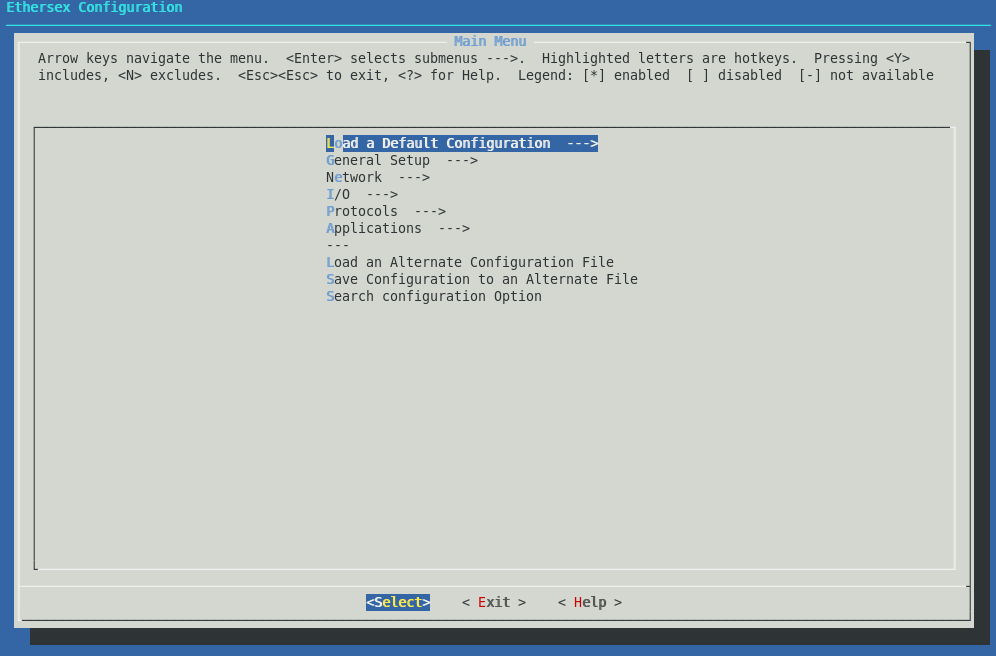
\includegraphics[width=10cm]{Main.png}
}
\frame{
  \frametitle{Modulauswahl}
  Menuconfig: Generelle Einstellungen
  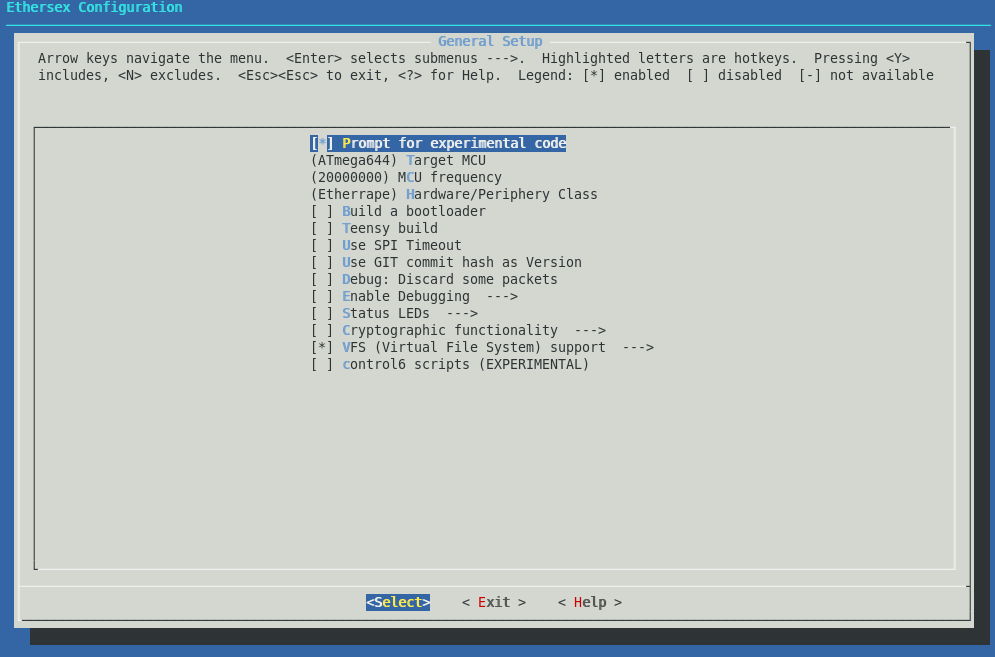
\includegraphics[width=10cm]{General.png}
}

\subsection{Unterstütze Hardware}
\frame{
  \frametitle{Unterstütze Hardware}
  \begin{block}<1->{Bausätze}
    \begin{itemize}
      \item Etherrape (fd0;lochraster.org)
      \item Net-IO (Pollin)
      \item AVR-Webserver (U. Radig)
      \item Thermotronic Basic (Eurotronic) \\Thermy (Aldi)
      \item ProBot (Conrad)
    \end{itemize}
  \end{block}
}

\subsection{Eigene Hardware}
\frame{
  \frametitle{Eigenes Hardware Pinning}
  \begin{itemize}
   \item scripts/add-hardware NAME aufrufen
  \end{itemize}
  \pause
  %TODO Bild mit menuconfig (Hardware Auswahlmenue) und neuem Pinning
  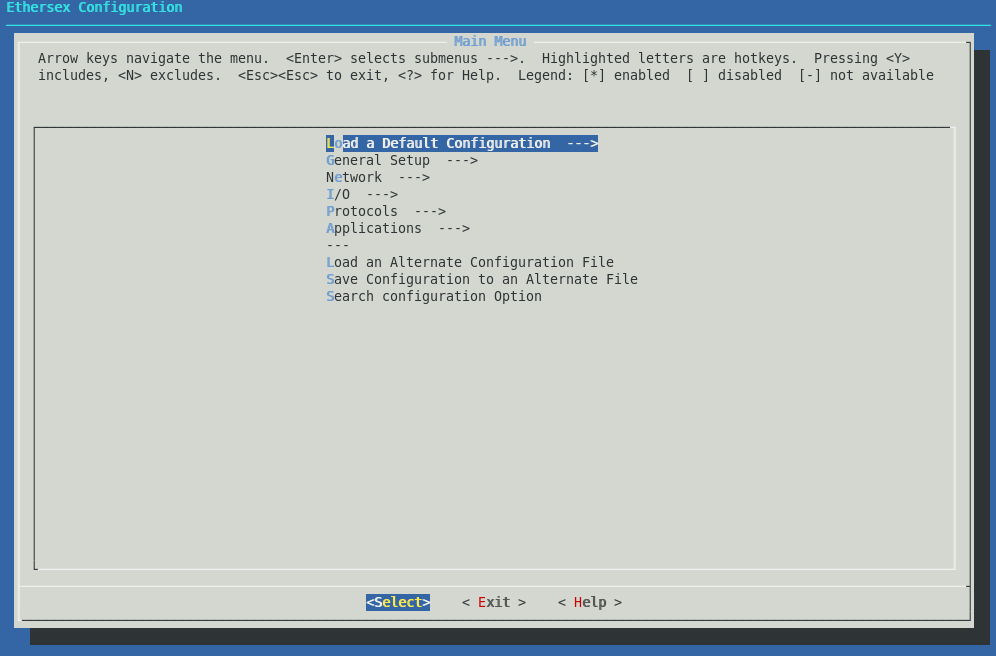
\includegraphics[width=10cm]{Main.png}
}

\section{Für Ethersex entwicklen}
%TODO Hier evtl. Mailingliste, Bugtracker erwähnen
\frame{
  \frametitle{Kontakt}
  TODO Hier evtl. Mailingliste, Bugtracker erwähnen
}

%TODO Hier github Fork Mechanismus 
\subsection{Git}
\frame{
  \frametitle{Git Fork}
  TODO Hier github Fork Mechanismus 
}

%TODO Metaschicht, Control6, EIngebettete Seite, Ecmd
\subsection{Modul hinzufügen}
\frame{
  \frametitle{Eigenes Modul hinzufügen}
    Metaschicht?\\
    Control6?\\
    Eingebette Webseite\\
    Ecmd
}

\section{Fragen}
\frame{
\frametitle{www.ethersex.de}
Fragen? \\
Anregungen? \\
\bigskip 
\bigskip 
\bigskip 
\begin{center}
\textbf{Danke für die Aufmerksamkeit!}\end{center}
\bigskip 
\bigskip 
\bigskip 
\begin{center}
 \begin{small}Projekt-Wiki: \texttt{www.ethersex.de}\\ Vortragsfolien: \texttt{www.ethersex.de/index.php/Kurzvortrag} \end{small}
\end{center}
}
\end{document}
